\subsection{Statistical quality of the SAA solutions}\label{sec:saa}

How many scenarios are enough?
For a regular day (5 March 2026) and for Black Friday 2025 we solve $M=10$ independent SAA replications for each $N\in\{10,25,50,100,200,400\}$, with scenarios from the true distribution.
Every resulting plan is evaluated on the same 5000 fresh scenarios.
Following \citet{mak1999}:
\begin{itemize}
  \item the mean of the $M$ SAA optimal values is a statistical \emph{lower} bound on the true optimum (in expectation), with a $t$-based confidence interval;
  \item the best out-of-sample value is an \emph{upper} bound.
\end{itemize}

\begin{table}[t]
\centering\small
\caption{SAA bounds ($M=10$ replications per $N$, out-of-sample evaluation on 5000 true scenarios). Gap CI: 95\% upper confidence bound on the optimality gap of the best plan, $(\mathrm{UB}-\mathrm{LB}+\mathrm{hw})/\mathrm{UB}$. Time: mean Benders solve time (24 workers).}\label{tab:saa}
\resizebox{\linewidth}{!}{\begin{tabular}{@{}lrrrrrrr@{}}\toprule
Day & $N$ & Lower bound (95\% CI) & Best UB & Mean UB & Gap (\%) & Gap CI (\%) & Time (s) \\ \midrule
\multirow{6}{*}{2025-11-28} & 10 & 4{,}609{,}718 $\pm$ 61{,}195 & 4{,}609{,}066 & 4{,}611{,}047 & -0.014 & 1.314 & 0.5 \\
 & 25 & 4{,}608{,}203 $\pm$ 28{,}740 & 4{,}609{,}334 & 4{,}609{,}642 & 0.025 & 0.648 & 0.4 \\
 & 50 & 4{,}609{,}204 $\pm$ 15{,}447 & 4{,}608{,}596 & 4{,}609{,}259 & -0.013 & 0.322 & 0.7 \\
 & 100 & 4{,}608{,}588 $\pm$ 16{,}167 & 4{,}607{,}959 & 4{,}609{,}119 & -0.014 & 0.337 & 1.2 \\
 & 200 & 4{,}611{,}299 $\pm$ 15{,}916 & 4{,}608{,}849 & 4{,}609{,}101 & -0.053 & 0.292 & 1.9 \\
 & 400 & 4{,}604{,}010 $\pm$ 9{,}490 & 4{,}608{,}717 & 4{,}608{,}990 & 0.102 & 0.308 & 3.9 \\
\midrule
\multirow{6}{*}{2026-03-05} & 10 & 2{,}288{,}673 $\pm$ 27{,}928 & 2{,}290{,}941 & 2{,}292{,}870 & 0.099 & 1.318 & 11.8 \\
 & 25 & 2{,}288{,}738 $\pm$ 13{,}196 & 2{,}290{,}634 & 2{,}291{,}043 & 0.083 & 0.659 & 7.0 \\
 & 50 & 2{,}289{,}886 $\pm$ 6{,}882 & 2{,}290{,}485 & 2{,}290{,}697 & 0.026 & 0.327 & 14.9 \\
 & 100 & 2{,}289{,}350 $\pm$ 7{,}560 & 2{,}290{,}383 & 2{,}290{,}584 & 0.045 & 0.375 & 17.5 \\
 & 200 & 2{,}291{,}186 $\pm$ 7{,}021 & 2{,}290{,}276 & 2{,}290{,}469 & -0.040 & 0.267 & 30.2 \\
 & 400 & 2{,}288{,}141 $\pm$ 4{,}345 & 2{,}290{,}262 & 2{,}290{,}520 & 0.093 & 0.282 & 30.4 \\
\bottomrule\end{tabular}
}
\end{table}

\begin{figure}[t]
  \centering
  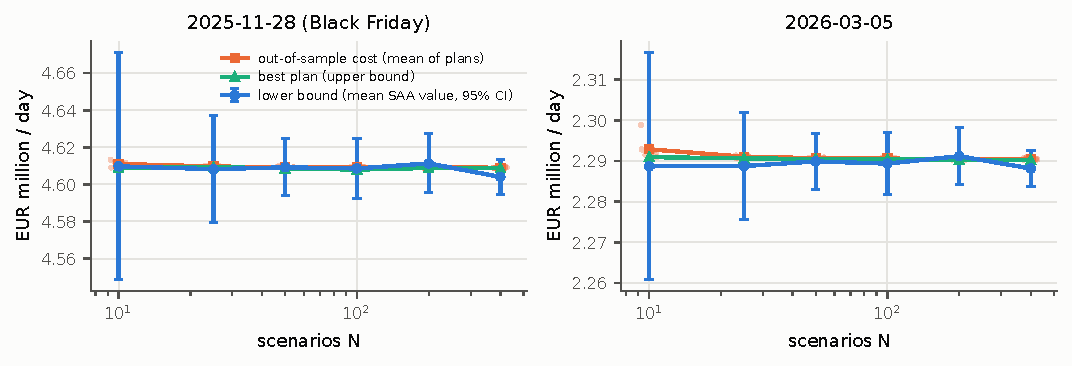
\includegraphics[width=\linewidth]{saa}
  \caption{SAA convergence. The plans' true expected cost (orange) stabilises from $N\approx 50$; the lower-bound estimator (blue, 95\% CI) tightens around it as $N$ grows.}
  \label{fig:saa}
\end{figure}

\Cref{tab:saa,fig:saa} show that the planning problem is statistically well behaved.
\begin{itemize}
  \item The true expected cost of the SAA plans stabilises quickly. Its spread across replications falls from \EUR{2239} per day at $N=10$ to about \EUR{140} at $N\ge 50$, and the plans at $N=100$ and $N=400$ differ by only \EUR{64} per day.
  \item The estimated optimality gap is statistically indistinguishable from zero for all $N\ge 25$. Its 95\% upper confidence bound falls to 0.3--0.4\% at $N\ge 50$, a level limited by the variance of the lower-bound estimator, not by the quality of the plans.
\end{itemize}
We therefore use $N=100$ throughout. Note also the optimisation tolerance of $5\cdot10^{-4}$ (\cref{sec:benders}): it is of the same order as these statistical errors, so solving more tightly would be pointless.

\paragraph{Value of the stochastic solution and of perfect information.}
\begin{table}[t]
\centering\small
\caption{Value of the stochastic solution (VSS $=$ EEV $-$ RP, paired over 5000 scenarios, $\pm$ 95\% CI) and expected value of perfect information (EVPI $=$ RP $-$ WS over 100 scenarios). RP: stochastic plan; EEV: plan for the mean demand; WS: wait-and-see.}\label{tab:vss}
\resizebox{\linewidth}{!}{\begin{tabular}{@{}lrrrrrrrr@{}}\toprule
Day & RP & EEV & VSS & WS & EVPI & Unmet \% & Trucks & Crews \\
 & \EUR{}/day & \EUR{}/day & \EUR{}/day & \EUR{}/day & \EUR{}/day & RP / EEV & RP / EEV & RP / EEV \\ \midrule
2026-03-05 & 2{,}290{,}262 & 2{,}293{,}459 & 3{,}196 $\pm$ 159 & 2{,}273{,}811 & 22{,}698 $\pm$ 2{,}602 & 0.12 / 0.03 & 519 / 530 & 252 / 257 \\
2025-11-28 & 4{,}607{,}959 & 4{,}615{,}030 & 7{,}071 $\pm$ 230 & 4{,}607{,}093 & 18{,}130 $\pm$ 1{,}590 & 0.79 / 0.77 & 954 / 952 & 425 / 425 \\
\bottomrule\end{tabular}
}
\end{table}

\Cref{tab:vss} decomposes the value of information.
\begin{itemize}
  \item \textbf{VSS.} The stochastic plan saves \EUR{3.2}k per day on the regular day and \EUR{7.1}k on Black Friday over the plan for mean demand. This is small (0.14\% and 0.15\%) but highly significant.
  \item \textbf{EVPI.} Perfect information would be worth \EUR{18}--\EUR{23}k per day, six to seven times more. Better \emph{information}, i.e.\ forecasts, matters more than better \emph{modelling of uncertainty}, consistent with \cref{sec:value-forecast}.
  \item \textbf{Direction of the hedge.} The SP plan buys \emph{fewer} trucks (519 vs.\ 530) and crews (252 vs.\ 257) than the mean-value plan. This is the newsvendor logic. Scheduled capacity costs $c$ and its same-day substitutes cost $1.6c$ (overtime) and $1.8c$ (spot), so the critical ratio $(1.8c-c)/(1.8c)\approx0.44$ is below one half. It is optimal to plan \emph{below} the mean and buy flexibility on the day. A planner who reasons only in terms of point forecasts would build the opposite safety margin. On Black Friday the labour limits bind (425 of 426 crews), so the hedge acts on trucks only.
\end{itemize}
